\documentclass[11pt]{amsart}

\usepackage{amsmath}
\usepackage{amsfonts}
\usepackage{amsthm}

\usepackage{showlabels}

\usepackage{tikz}
\usetikzlibrary{arrows}

\usepackage{lipsum}

\usepackage{listings}

\usepackage{enumerate}

\lstset{basicstyle=\ttfamily, mathescape=true}

\newcommand{\R}{\mathbb{R}}
\newcommand{\Q}{\mathbb{Q}}
\newcommand{\Z}{\mathbb{Z}}
\newcommand{\N}{\mathbb{N}}
\newcommand{\HH}{\mathcal{H}}
\newcommand{\BB}{\mathcal{B}}

\newtheorem{lemma}{Lemma}
\newtheorem{theorem}{Theorem}
\newtheorem{corollary}{Corollary}
\newtheorem{prop}{Prop}

\newtheorem{definition}{Definition}

\newtheorem{conjecture}{Conjecture}

\newtheorem{remark}{Remark}

\DeclareMathOperator{\dig}{dig}
\DeclareMathOperator{\intr}{int}


\DeclareMathOperator{\len}{le}
\newcommand{\LE}{\mathbf{LE}}

\title[\textbf{Optimal bounds for $b$-ary measures}]{\textbf{On optimal bounds for comparing Binary (and $b$-ary) Nest Measures with the Hausdorff Measure on $\R$}}


\author{Duarte Maia}
\address{Department of Mathematics, Instituto Superior Técnico}
\email{duarte.nascimento@tecnico.ulisboa.pt}

\iffalse

\author{Jorge Drumond Silva}
\address{Department of Mathematics, Instituto Superior Técnico}
\email{jsilva@math.ist.utl.pt}

\fi

\date{}


\begin{document}


\begin{abstract}
\lipsum[1]
\end{abstract}

\maketitle


\section{Introduction}

\lipsum[1]

\section{Hausdorff and Binary measures: a review}

\subsection{Hausdorff}

Let $X$ be a metric space, with distance $d$. We define the \emph{$s$-dimensional Hausdorff measure on $X$} as follows:

First, for $E \subseteq X$, $s \in \R^+_0$ and $\delta > 0$, define $\HH_s^\delta(E) := \inf \sum_i \lvert U_i \rvert^s$, where:

\begin{itemize}

\item $\lvert E \rvert$ denotes the \emph{diameter of $E$}, defined by the $\sup$ of distances between elements of $E$;\footnote{We follow the convention that the diameter of the empty set be 0.}

\item The infimum is taken over countable coverings $\{U_i\}_{i \in \N}$ of $E$ such that the diameter of all $U_i$ is less than $\delta$. This is usually abbreviated to `$U$ is a \emph{$\delta$-covering}'.

\end{itemize}

As $\delta$ decreases this quantity increases. Hence, the limit $\lim_{\delta \to 0} \HH_s^\delta(E)$ exists in $\left[ 0, \infty \right]$. It is this quantity that we call the \emph{$s$-dimensional Hausdorff measure of $E$}:

\begin{definition}(Hausdorff Measure)

 \[\HH_s(E) := \lim_{\delta \to 0} \HH_s^\delta(E)\]
\end{definition}

\subsection{Dimension}

Fixed any set $E$ in a metric space $X$, there exists a dimension $\sigma \in \left[0, \infty\right]$ such that:

\begin{itemize}
\item For $s < \sigma$, $\HH_s(E) = \infty$;

\item For $s > \sigma$, $\HH_s(E) = 0$;
\end{itemize}

To aid with the proof, we introduce the following lemma:

\begin{lemma}\label{helperdimension}
Let $t < s$ be real nonnegative numbers. Then, if $\HH_t(E) < \infty$ we have $\HH_s(E) = 0$.
\end{lemma}

\begin{proof}
Suppose $t < s$ and $\HH_t(E) < \infty$. Put $M = \HH_t(E) + 1$. Then, for any $\delta > 0$ we may find a $\delta$-covering $\{U_i\}$ of $E$ such that $\sum \lvert U_i \rvert^t < M$. Hence, 

\begin{align*}
\sum \lvert U_i \rvert^s &= \sum \lvert U_i \rvert^t \lvert U_i \rvert^{s - t}\\
&\leq \sum \lvert U_i \rvert^t \delta^{s-t}\\
&\leq \delta^{s-t} M
\end{align*}

Therefore, $\HH_s^\delta(E) \leq \delta^{s-t} M$, and so making $\delta \to 0$ we get $\HH_s(E) = 0$, as desired.
\end{proof}

We can now define, the dimension of a set $E$.

\begin{definition} (Hausdorff dimension of a set)

\[\sigma_E := \inf \{\, s \mid \HH_s(E) < \infty \,\}\]
\end{definition}

\begin{prop}
(Well-definedness of the dimension of a set) Let $E \subseteq X$, where $X$ is a metric space.

\begin{itemize}
\item For $s < \sigma_E$, $\HH_s(E) = \infty$;

\item For $s > \sigma_E$, $\HH_s(E) = 0$;
\end{itemize}

\end{prop}

\begin{proof}
The first inequality is trivial by definition of $\sigma_E$.

To show the second inequality, notice that if $s > \sigma_E$ then there exists $t < s$ such that $\HH_t(E) < \infty$. By lemma \ref{helperdimension}, we have $\HH_s(E) = 0$, as desired.
\end{proof}

This shows that the dimension of a set is the only dimension for which its Hausdorff measure may be nontrivial, that is, different from $0$ or $\infty$.

\begin{definition}
We will say $E \subseteq X$ is an \emph{$s$-set} if $\HH_s(E) \in \left]0, \infty \right[$.
\end{definition}

\subsection{Net measures}

Hausdorff measure, and by extension Hausdorff dimension, is often very difficult to compute precisely as its definition requires one to look at all possible $\delta$-coverings. As such, there is interest in finding definitions that would allow simpler methods of computing, or at least estimating, these quantities.   

We will restrict our attention to $\R^n$, and later on to $\R$, as a lot of what follows is not immediately generalizable to other contexts.

First, notice that it is not uncommon for one to restrict their attention to specific coverings. Indeed, if in the definition of $\HH_s^\delta$ one takes the infimum over \emph{open} $\delta$-coverings instead of arbitrary ones, the value of $\HH_s^\delta$ may change, but the limit as $\delta \to 0$ remains the same. Hence, one could consider the Hausdorff measure defined using open $\delta$-coverings with no loss of generality.

The notion of net measure arises from the idea of redefining the Hausdorff measure with a more manageable collection of sets to use for coverings. In the context of $\R^n$, Besicovitch (1952) used the so-called binary intervals, construction which we will make solely for the case of $n = 1$, but more exhaustive treatments can be found in \cite{falconer} \cite{rogers}.

\begin{definition}
Define the so-called \emph{binary intervals} in $\R$ as the set of intervals of the form $\left[ k 2^j, (k+1) 2^j \right[$, for $k, j \in \Z$.

The binary measure is defined analogously to the Hausdorff measure, except instead of arbitrary coverings one restricts themselves to $\delta$-coverings by binary intervals. It is denoted by $\BB_s(E) = \lim_{\delta \to 0} \BB_s^\delta(E)$.
\end{definition}

The usefulness of this definition lies in that, even though these measures do \emph{not} coincide in general with the Hausdorff measure, one can find bounds for one given the other.

The following theorem is found in \cite{falconer} \cite{rogers} and is left here without proof, though in the sequence of this document we will prove stronger results for the particular case of $n = 1$.

\begin{theorem}\label{badbound}
Consider the Hausdorff and Binary measures defined in $\R^n$. The following inequalities hold for any set $E$:

\[ \HH_s(E) \leq \BB_s(E) \leq 3^n 2^{n^2} \HH_s(E) \]
\end{theorem}

\begin{remark}
Even though the preceding theorem will not be proven, it should be noticed that one of the inequalities is trivial.

Indeed, for any $\delta$ we have $\HH_s^\delta(E) \leq \BB_s^\delta(E)$, since both are infima taken over coverings of $E$, but the set of coverings `accepted' by the Hausdorff measure is a superset of those considered in the binary measure. Making $\delta \to 0$, we have inequality $\HH_s(E) \leq \BB_s(E)$.
\end{remark}

The preceding theorem has the following consequence: defining the ``binary dimension'' of a set analogously to how we defined the Hausdorff dimension, these two concepts would coincide. Indeed, the Hausdorff measure of a set is zero iff the binary measure is zero, and same for infinity.

Hence, if we are interested in the Hausdorff dimension of a set, we may begin by investigating its binary measure.

Notice, however, that the provided bound is not very sharp. Indeed, for $n = 1$ the obtained constant amounts to 6, but we will see below that it can be significantly lowered without much effort. (And then lowered more, with significantly more effort.)

Of course, this is of no consequence for dimensional considerations, which is where (as far as the author is aware) their main utility is found. However, the results that follow allow for much tighter bounds, and hopefully better understanding of how these two relate.

\subsection{Hausdorff Coverings}

As mentioned above, it is sometimes convenient, yet entirely admissible, for one to only consider open coverings of sets instead of allowing for the full generality of any possible covering. This is not the only simplification that will be useful for us to do.

Notice that any monotone operation that can be done on a set without increasing its diameter can be assumed to be done without loss of generality.

To use an example: notice that taking the closure of a set $U$ does not increase its diameter. As such, given any $\delta$-covering $\{U_i\}$ of a set $E$, the collection $\{ \overline{U_i} \}$ is also a $\delta$-covering of $E$, with all sets closed, and with all diameters the same, whence the Hausdorff sum is also the same. This shows, then, that we can assume without loss of generality that our infimum in the definition of $\HH_s^\delta$ can be taken over the closed sets.

A more specific example, yet useful for our purposes, is (in $\R^n$) the operation of taking the convex hull, which satisfies the condition of monotony and not increasing diameters. This shows, then, that we may take infima over convex sets with no loss of generality.

In the particular case of $\R$, what this shows is that we can assume the sets we are using for coverings are intervals. Sometimes it will be useful for us to assume these intervals closed, sometimes it is useful to suppose them open. In any case, the reader should be aware that these hypotheses harm in no way the generality of the results obtained.

As a final remark, it is often useful to exclude, in our coverings, cases where the sets have diameter 0. Indeed, many authors explicitly exclude the case of 0-diameter sets in the definition of $\delta$-coverings.

\section{Better elementary bounds}

We have already shown that, in $\R$, $\HH_s \leq \BB_s$. We will now proceed to establish a bound in the opposite direction, beginning our journey to find optimal bounds.

Everything that follows will be done in the context of $\R$.

\begin{theorem}
\[ \BB_s \leq 3 \HH_s \]
\end{theorem}

\begin{proof}
To show this fact, we will show that for any $E$ and $\delta$ we have the inequality $\BB_s^\delta(E) \leq 3 \HH_s^\delta(E)$. To this effect, we will show that given any $\delta$-covering of $E$ we can construct a binary $\delta$-covering of $E$ such that its `Hausdorff sum' is not much bigger than the original's.

Fix, then, a $\delta$-covering $\{U_i\}$ of $E$, which we suppose without loss of generality to be composed of intervals with diameter strictly greater than zero. Define, for each $i$, $j_i$ to be the greatest integer such that $2^{j_i} < \lvert U_i \rvert$, and hence $2^{j_i} < \delta$ for all $i$.

Notice that at least one interval of the form $\left[ k_i 2^{j_i}, (k_i + 1) 2^{j_i} \right[$ is wholly contained within $U_i$. Furthermore, this interval, united with the intervals of its size immediately to its left and immediately to its right, cover $U_i$ entirely.

Now, consider the covering $\{I_i\}$ obtained from $\{U_i\}$ by replacing each $U_i$ by the three intervals mentioned above. We now have a binary $\delta$-covering of $E$, with Hausdorff sum:

\[\sum \lvert I_i \rvert^s \leq 3 \sum \lvert U_i \rvert^s\]

This inequality because for every $U_i$ we assign its three corresponding intervals, each with diameter less than $\lvert U_i \rvert$. This completes our proof, since:

\begin{align*}
3 \HH_s^\delta &= 3 \times \inf \text{over $U_i$}\\
&\geq \inf \text{over the corresponding $I_i$}\\
&\geq \inf \text{over all binary $\delta$-coverings}\\
&= \BB_s^\delta
\end{align*}

\end{proof}

This bound, while twice as sharp as the one mentioned in theorem \ref{badbound}, can still be significantly improved. The proof, however, touches on what will be our main tool to try to control the bound. The idea is to find a way to replace any $\delta$-covering with a binary $\delta$-covering such that, if the first covering has Hausdorff sum $A$, the latter has Hausdorff sum at most $CA$, where $C$ is the bound we desire to prove. Taking this a step further, we can focus merely on finding a way to, given an interval of length $\ell$, covering it by binary intervals of lengths $m_i$ such that $\sum m_i^s \leq C \ell^s$. One might have concerns about making sure that these binary intervals still form a $\delta$-covering, but that is not an issue, as we will see in the following lemma:

\begin{lemma}
Fix a dimension $s \in \R^+$.

Suppose $C \in \R^+$ is such that, for any interval $I$ of length $\ell$, we can find a countable binary covering of $I$ by intervals $\{J_i\}$ of lengths $m_i$ such that

\[\sum m_i^s \leq C \ell^s\]

Then $\BB_s \leq C \HH_s$.
\end{lemma}

\begin{proof}
This proof proceeds much like the previous one, with one caveat.

Fixed some $E$, let $I_i$ be any $\delta$-covering of $E$ by intervals. For each $I_i$, let $\{J_{ij}\}_{j \in \N}$ be a collection of binary intervals such that  $\sum_j \lvert J_{ij} \rvert^s \leq C \lvert I_i \rvert^s$.

First, notice that, while it is \emph{not} necessarily true that the collection $\{J_{ij}\}_{i,j \in \N}$ forms a $\delta$-covering, we can be assured that it forms at most a $C^{1/s}\delta$-covering, as, for any $i, j$ we have

\[ \lvert J_{ij} \rvert^s \leq \sum_j \lvert J_{ij} \rvert^s \leq C \lvert I_i \rvert^s \leq C \delta^s\]

And so $\lvert J_{ij} \rvert \leq C^{1/s} \delta$, as desired.

The argument now goes much like the previous one, except we can only show that $\BB_s^{C^{1/s} \delta} \leq C \HH_s^\delta$. This turns out to be enough, however, as taking $\delta \to 0$ also yields $C^{1/s} \delta \to 0$, and so both sides of this inequality converge to $\BB_s$ and $\HH_s$, respectively.
\end{proof}

\begin{remark} \label{dimnotzero}
We had to exclude the case $s = 0$ from consideration in this last proposition, as we will have to in a lot of what follows. This is a nonissue, however, as this particular case is extremely easy to examine. Indeed, for this dimension both the Hausdorff and the binary measure turn out to be simply the counting measure on the reals.

As such, in all that follows, unless said otherwise, \textbf{it should be assumed that $s \neq 0$}.
\end{remark}

This previous lemma will be central in what follows. Indeed, our strategy to find a bound $C$ will be to, given any interval $I$, find a binary covering $\{J_i\}$ of $I$ such that $\sum \lvert J_i \rvert^s \leq C \lvert I \rvert^s$. But before moving on, a few remarks are in order.

\section{$b$-ary measures}

As mentioned before, for the purposes of dimensional analysis, the binary measures are more than sufficient. However, for the purposes of estimating the Hausdorff measure, it might be worth looking into something slightly more general than binary intervals.

\begin{definition}
Define the $b$-ary intervals, where $b \in \Z_{\geq 2}$, as those of the form:

\[\left[k b^j, (k+1) b^j \right[, \;k, j \in \Z\]

The definition for the $s$-dimensional $b$-ary measure, denoted $\BB_{bs}$, and the corresponding $\delta$-measures $\BB_{bs}^\delta$, should be evident by comparison to the definition of the binary one, using the $b$-ary intervals instead of the binary ones.
\end{definition}

The results of the last section can be translated into this slightly more generic context without much added effort. We leave the results here without proof.

\begin{lemma}
Fix a dimension $s \in \R^+$ and a base $b \in \N_{\geq 2}$.

Suppose $C \in \R^+$ is such that, for any interval $I$ of length $\ell$, we can find a countable $b$-ary covering of $I$ by intervals $\{J_i\}$ of lengths $m_i$ such that

\[\sum m_i^s \leq C \ell^s\]

Then $\BB_{bs} \leq C \HH_s$.

In particular, one can easily show the premise is true for $C = b+1$, whence one gets the bound:

\[\HH_s \leq \BB_{bs} \leq (b+1) \HH_s\]
\end{lemma}

This last bound hints at something we will study: it appears that, the bigger the $b$ (that is, the more pieces we divide our intervals in) the worse the estimate. This makes sense: the bigger the $b$, the less we can discern because since there is a larger discrepancy between the size of one layer and the next we lose the ability to gauge more precisely the intermediate sizes.

This intuition proves to be partially correct, as the following proposition shows:

\begin{prop}
Let $b, c \in \Z_{\geq 2}$ and suppose $c$ is a multiple of $b$.

Then, $\BB_{bs} \leq \BB_{cs}$
\end{prop}

\begin{proof}
This proof is trivial: simply notice that, if $c$ is a multiple of $b$, any $c$-ary interval is also a $b$-ary one. As such, when taking the infima for $\BB_{bs}^\delta$ one has more sets than in $\BB_{cs}^\delta$, whence $\BB_{bs}^\delta \leq \BB_{cs}^\delta$ and the result follows.
\end{proof}

We conjecture that this proposition captures precisely which of these measures are greater than others. That is:

\begin{conjecture}
$\BB_{bs} \leq \BB_{cs}$ iff $c$ is a multiple of $b$.
\end{conjecture}

Unfortunately, we have, as of yet, been unable to show this. We do, however, have some evidence that shows that the following proposition is \textbf{false}: 

\begin{conjecture}
If $c \geq b$ then $\BB_{bs} \leq \BB_{cs}$.
\end{conjecture}

The counterexample to this possible conjecture is found closer to the end of this document.

\section{Minimal interval coverings}

We focus now on the problem of, fixed a dimension $s$ and given an interval $I$, finding a $b$-ary covering of $I$ with as small a Hausdorff sum as possible. We assume $I$ to be of the form $\left[ a, b \right[$ with $a < b$, as we can always assume our Hausdorff coverings are composed of intervals of this kind. The reason we are assuming this is so that this plays well with our binary intervals, which are also half-open.

In truth, what we are actually concerned about is, as a function of the length of the interval $I$, let's call it $\ell$, how small a $b$-ary covering of it can we make? In particular, we want to find out the smallest $C$ such that we can always find a binary covering with Hausdorff sum less than or equal to $C \ell^s$. Symbolically this can be written as:

\[\sup \frac{\BB_{bs}^\infty(I)}{\lvert I \rvert^s}\]

Where the supremum is taken over the half-open nonempty intervals $I$ and the usage of $\delta = \infty$ is intended to imply that any binary covering is admissible.

Notice, now, that an interval is uniquely determined by its length and its position. We can, then, write that supremum as:

\[\sup_\ell \sup_\text{$I$ of length $\ell$} \frac{\BB_{bs}^\infty(I)}{\ell^s}\]

Which is the same as:

\[\sup_\ell \frac{\sup_I \BB_{bs}^\infty(I)}{\ell^s}\]

We investigate, then, $\sup \BB_{bs}^\infty(I)$, where the supremum is taken over intervals of a fixed length $\ell$.

We will now show the following: we can assume, in addition, that our interval contains the origin. To this effect, given any interval $I$ we will construct an interval $I'$ of same length containing the origin, such that $\BB_{bs}^\infty(I') \geq \BB_{bs}^\infty(I)$.

This construction requires splitting into cases:

Let $\ell = \lvert I \rvert$, and $j$ such that $b^j < \ell \leq b^{j+1}$.

Does there exist a number of the form $k b^{j+1}$ contained in $I$?
%%Todo make explicit that s \in ]0,1]
\begin{enumerate}

\item \textbf{If so,} let $I'$ be the interval given by translating $I$ by $-k b^{j+1}$. Two easy observations are in order. Observation number one:

\[\BB_{bs}^\infty(I') = \BB_{bs}^{b^{j+1}}(I')\]

This is clearly true because any covering of $I'$ using an interval of size greater than $b^{j+1}$ can be `improved' by replacing it with a smaller interval. Observation number two:

\[\BB_{bs}^{b^{j+1}}(I') = \BB_{bs}^{b^{j+1}}(I)\]

This is clearly true because the translation done to turn $I$ into $I'$ preserves binary intervals of size $b^{j+1}$ or less.

These two, joined with the fact that $\BB_{bs}^{b^{j+1}}(I) \geq \BB_{bs}^\infty(I)$, give us the desired inequality:

\[\BB_{bs}^\infty(I') \geq \BB_{bs}^\infty(I)\]

\item \textbf{If not,} then we have

\[\BB_{bs}^\infty(I) = \min(\BB_{bs}^{b^j}(I), b^{(j+1)s})\]

We know for sure there exists at least one point of the form $k b^j$ in $I$. Let $I'$ be given by translating $I$ by $-k b^j$. We proceed to compare $\BB_{bs}^\infty(I')$ and $\BB_{bs}^\infty(I)$.

\begin{enumerate}

\item \textbf{If} $\BB_{bs}^{b^j}(I) \leq b^{(j+1)s}$, then notice that, as above, we have

\[\BB_{bs}^{b^j}(I') = \BB_{bs}^{b^j}(I) \leq b^{(j+1)s}\]

And thus, $\BB_{bs}^{b^j}(I') = \BB_{bs}^\infty(I')$, as any coverings containing intervals bigger then $b^j$ can be safely ignored. Finalizing, we get:

\[\BB_{bs}^\infty(I') = \BB_{bs}^{b^j}(I') = \BB_{bs}^{b^j}(I) = \BB_{bs}^\infty(I)\]

\item \textbf{If} $\BB_{bs}^{b^j}(I) \geq b^{(j+1)s}$, simply observe that either

\[\BB_{bs}^\infty(I') = \BB_{bs}^{b^j}(I')\]

In which case $\BB_{bs}^\infty(I') = \BB_{bs}^{b^j}(I) \geq \BB_{bs}^\infty(I)$, as desired.

Or it could happen that

\[\BB_{bs}^\infty(I') < \BB_{bs}^{b^j}(I')\]

In which case we can safely assert $\BB_{bs}^\infty(I') \geq b^{(j+1)s} = \BB_{bs}^\infty(I)$ since we need only consider coverings that contain at least one interval of length $b^{j+1}$ and so have Hausdorff sum of at least $b^{(j+1)s}$.
\end{enumerate}
\end{enumerate}

\qed

This construction done, we have now shown that our problem can be reduced to


\[\sup_{\substack{\text{$I$ half-open interval}\\ 0 \in I}} \frac{\BB_{bs}^\infty(I)}{\lvert I \rvert^s}\]

A simple observation about the origin is that any $b$-ary interval is either to the right or to the left of the origin, but no interval touches both sides. As such, we can consider our covering of the left side to be independent of our covering of the right side, leading quickly to the conclusion that, if $I = \left[ a, b \right[$ with $a \leq 0 \leq b$, we have:

\[\BB_{bs}^\delta(\left[a, b\right[) = \BB_{bs}^\delta(\left[a, 0\right[) + \BB_{bs}^\delta(\left[0, b\right[)\]

For any $\delta \in \left]0, \infty \right]$.

Another observation, which we will justify rigorously soon (see lemma \ref{sidedoesntmatter}), is that $\BB_{bs}^\delta(\left[a, 0\right[) = \BB_{bs}^\delta(\left[0, a\right[)$. This has the following consequence: if we define for $t \geq 0$ the function $g_{bs}(t) := \BB_{bs}^\infty(\left[0, t \right[)$, our problem becomes one of optimization:

\[ \sup_{\substack{\ell,r \in \R^+_0\\\ell+r \neq 0}} \frac{g_{bs}(\ell) + g_{bs}(r)}{(\ell + r)^s} \]

And so, we proceed to study the function $g_{bs}$, (we will often suppress the subscript when it is obvious from context and not particularly relevant) which has a connection to the theory of $b$-ary expansions of real numbers. Before going into details, however, the promised lemma:

\begin{lemma} \label{sidedoesntmatter}
\[\BB_{bs}^\delta(\left[a, 0\right[) = \BB_{bs}^\delta(\left[0, a\right[)\]
\end{lemma}

\begin{proof}
Fix any $b$-ary $\delta$-covering of $\left[a, 0\right[$. Suppose it is $\{\left[x_i, y_i\right[\}$. Consider the collection $\{\left[-y_i, -x_i\right[\}$. 

This collection almost forms a $b$-ary $\delta$-covering of $\left[0, a\right[$. Indeed, the only points that might not be covered are those of the form $-x_i$, but one may easily augment our collection of intervals with things of the form $\left[ -x_i, -x_i + \varepsilon_i \right[$ with arbitrarily small $\varepsilon_i$, and so reach the conclusion that there are coverings of $\left[0, a\right[$ with Hausdorff sum arbitrarily close to our original covering's, concluding that $\BB_{bs}^\delta(\left[a, 0\right[) \geq \BB_{bs}^\delta(\left[0, a\right[)$. The same argument works to get the other inequality, and thus we get the desired equality.
\end{proof}

\section{$b$-ary digit expansions}

In the previous section we showed that a possible approach to our problem goes through investigating the optimization problem:

\[ \sup_{\substack{\ell,r \in \R^+_0\\\ell+r \neq 0}} \frac{g_{bs}(\ell) + g_{bs}(r)}{(\ell + r)^s} \]

By itself, this reduction would not be much help, but as it turns out one can draw a connection between this function $g$ and the theory of noninteger base expansions.

\begin{remark}
In remark \ref{dimnotzero} we mentioned that we will be tacitly assuming $s \neq 0$. We will outline here another such assumption.

$\R$ has Hausdorff dimension 1. As such, for $s > 1$, both the binary and the Hausdorff measre of \emph{any} set in $\R$ will be zero. Then, the question of the relationship between these two is trivial and uninteresting. Therefore, we add another tacit assumption:

\textbf{From now on, we always assume $s \leq 1$.}
\end{remark}

Let us fix some $t > 0$, and investigate how one might go about calculating $g(t)$ fixed a dimension $s$ and a base $b$. (The case $t = 0$ is trivial, and thus unconsidered.) We remind the reader of the definition of $g$:

\[g_{bs}(t) := \BB_{bs}^\infty(\left[0, t \right[)\]

First, fix $b^k$ as the least power of $b$ that is $\geq t$. Then, a possible covering of $\left[0, t \right[$ would be the interval $\left[0, b^k\right[$. Hence, $g(t) \leq b^{ks}$.

Now, consider that $b^{k-1} < t$, and so there is a maximal integer, which we will call $d_1$, such that $d_1 b^{k-1} \leq t$. As such, this gives us another possible covering of our interval: consider the sequence of intervals formed by

\[\left[0, b^{k-1} \right[, \left[b^{k-1}, 2 b^{k-1} \right[, \cdots, \left[d_1 b^{k-1}, (d_1 + 1) b^{k-1} \right[ \]

This gives us another upper bound for $g(t)$: $g(t) \leq (d_1 + 1) b^{k-1}$.

We can continue this process: let $d_2$ be maximal such that $d_1 b^{k-1} + d_2 b^{k-2} \leq t$. The following sequence of intervals will cover $\left[0, t \right[$:

\begin{multline*}
\left[0, b^{k-1} \right[, \left[b^{k-1}, 2 b^{k-1} \right[, \cdots, \left[(d_1 - 1) b^{k-1}, d_1 b^{k-1} \right[ \\
\left[d_1 b^{k-1}, d_1 b^{k-1} + b^{k-1} \right[, , \cdots, \left[d_1 b^{k-1} + d_2 b^{k-2}, d_1 b^{k-1} + (d_2 + 1) b^{k-2} \right[
\end{multline*}

Giving us a new upper bound $d_1 b^{k-1} + (d_2 + 1) b^{k-2}$.

We will make this process more rigorous shortly. Below is a diagram exemplifying it for $b = 3$ and $t = 0.86$.


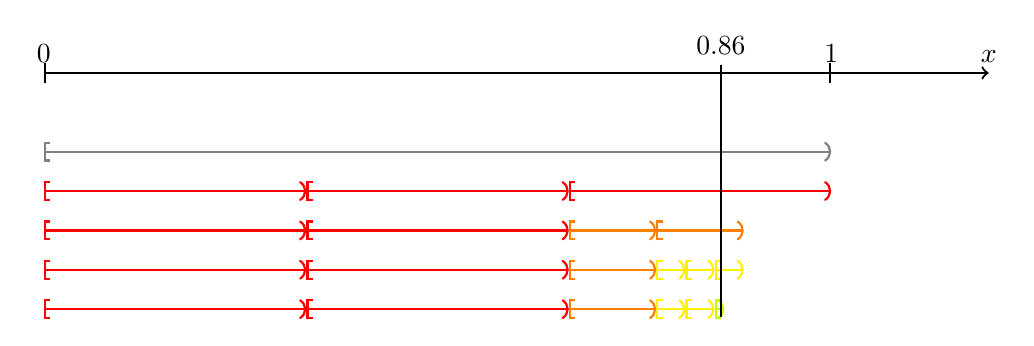
\begin{tikzpicture}
\draw[thick, {|-|}] (0,0) node[above]{0} -- (10,0) node[above]{1};
\draw[thick, {->}] (10,0) -- (12, 0) node[above]{$x$};

%The following was automatically generated with the help of the code at binary.py
\draw[thick, gray, {[-)}] (0, -1.0) -- (10, -1.0);
\draw[thick, red, {[-)}] (0, -1.5) -- (3.333333333333333, -1.5);
\draw[thick, red, {[-)}] (3.333333333333333, -1.5) -- (6.666666666666666, -1.5);
\draw[thick, red, {[-)}] (6.666666666666666, -1.5) -- (10.0, -1.5);
\draw[thick, red, {[-)}] (0, -2.0) -- (3.333333333333333, -2.0);
\draw[thick, red, {[-)}] (3.333333333333333, -2.0) -- (6.666666666666666, -2.0);
\draw[thick, orange, {[-)}] (6.666666666666666, -2.0) -- (7.777777777777777, -2.0);
\draw[thick, orange, {[-)}] (7.777777777777777, -2.0) -- (8.88888888888889, -2.0);
\draw[thick, red, {[-)}] (0, -2.5) -- (3.333333333333333, -2.5);
\draw[thick, red, {[-)}] (3.333333333333333, -2.5) -- (6.666666666666666, -2.5);
\draw[thick, orange, {[-)}] (6.666666666666666, -2.5) -- (7.777777777777777, -2.5);
\draw[thick, yellow, {[-)}] (7.777777777777777, -2.5) -- (8.148148148148147, -2.5);
\draw[thick, yellow, {[-)}] (8.148148148148147, -2.5) -- (8.518518518518515, -2.5);
\draw[thick, yellow, {[-)}] (8.518518518518515, -2.5) -- (8.888888888888886, -2.5);
\draw[thick, red, {[-)}] (0, -3.0) -- (3.333333333333333, -3.0);
\draw[thick, red, {[-)}] (3.333333333333333, -3.0) -- (6.666666666666666, -3.0);
\draw[thick, orange, {[-)}] (6.666666666666666, -3.0) -- (7.777777777777777, -3.0);
\draw[thick, yellow, {[-)}] (7.777777777777777, -3.0) -- (8.148148148148147, -3.0);
\draw[thick, yellow, {[-)}] (8.148148148148147, -3.0) -- (8.518518518518515, -3.0);
\draw[thick, lime, {[-)}] (8.518518518518515, -3.0) -- (8.641975308641975, -3.0);


\draw[thick] (8.6, 0.1) node[above]{0.86} -- (8.6, -3.1);
 
\end{tikzpicture}

\bigskip

Notice the structure of how we would find the $d_i$ in the previous argument: already knowing $d_1, \cdots, d_{i-1}$, one would pick $d_i$ as the maximal one such that $\sum_{j = 1}^i d_j b^{k-j} \leq t$. This is, in fact, the exact same algorithm used to find the $b$-ary digits of $t$.

So, let us consider the following algorithm to calculate $g(t)$:

Let $b^k$ be the least power of $b$ greater than $t$ for $t > 0$.

\begin{lstlisting}
$rem \leftarrow t$
$i \leftarrow 0$
Loop:
  $i \leftarrow i-1$
  Put $d_i$ be the greatest integer $k$ such that $k \cdot b^{k-i} \leq rem$
  $rem \leftarrow rem - d_i b^{k-1}$
\end{lstlisting}
\label{digalg}

The preceding algorithm will calculate the digits of $t$ in base $b$. Indeed, in base $b$, $t$ would be represented as:

\[d_1 d_2 \cdots d_k \, . \, d_{k+1} \cdots\]

Or, in scientific notation:

\[b^k \times 0.d_1 d_2 d_3 \dots\]

All the $d_i$ are members of the set $\{ 0, \cdots, b-1\}$, and furthermore we have:

\[\sum_{i = 1}^\infty d_i b^{k-i} = t\]

Finally, for any $N \geq 0$:

\[(\sum_{i=1}^N d_i b^{k-i}) + b^{k-N} \geq t\]

As such, we may consider the following sequence of intervals:

\begin{gather*}
\{\, \left[ x , x + b^{k-N} \right[ \mid x = (\sum_{i=1}^N d_i b^{k-i}) + j b^{k-N}, 0 \leq j < d_N, 0 \leq N \leq M\,\}\\
\cup\\
\{\left[ (\sum_{i=1}^M d_i b^{k-i}) ,(\sum_{i=1}^M d_i b^{k-i}) + b^{k-M} \right[\}
\end{gather*}

The notation has become extremely burdensome, so we make the following definitions:

\begin{definition}
First, we will use the notation $\left[ x, +\delta \right[$ to mean $\left[x, x+\delta \right[$.

Let $\{d_i\}_{i \in \N}$ be a sequence of natural numbers. Define the collection of intervals denoted by:

\[ b^k [d_0 d_1 d_2 \dots] \]

As follows:

First, define it inductively for finite sequences:

\begin{gather*}
b^k [] = \emptyset\\
b^k [d_0 \cdots d_n d_{n+1}] = b_n [d_0 \cdots d_n] \cup \{\,\left[d_0 . d_1 \cdots d_n j \times b^k, +b^{k-(n+1)} \right[ \mid 0 \leq j < d_{n+1} \,\}
\end{gather*}

And, for infinite sequences, simply take the increasing union:

\[ b^k[d_0 d_1 \dots] = \bigcup_{i = 0}^\infty b^k[d_0 \cdots d_i] \]

\end{definition}

The following propositions are left without proof.

\begin{prop}
Let $\{d_i\}_{i \in \N}$ be a sequence of natural numbers. Let $A = b^k [d_0 d_1 d_2 \dots]$. Then, $A$ satisfies the following properties:

\begin{itemize}
\item Every interval $I \in A$ is $b$-ary

\item $\cup_{I \in A} I = \left[ 0, t \right[$, where $t = b^k \times d_0 . d_1 d_2 \dots$

\item Every two intervals in $A$ are disjoint

\item The Hausdorff sum of $A$ is simply given by $b^{ks} \sum d_i b^{-is}$.
\end{itemize}

\end{prop}

\begin{remark}
Notice that the Hausdorff sum of $A$ can be easily written out as a $b^s$-ary expansion. Namely, $(b^s)^k \times d_0 . d_1 d_ 2 \dots$.

It is left implied when writing things with scientific notation that the base in which the expansion should be interpreted is the base of the mantissa. In this case, $b^s$. In the future, however, in this particular case, we will abbreviate it to $b^{ks}$, but the expansion following should still be interpreted as base $b^s$.
\end{remark}

This done, we can now more easily write down the coverings mentioned above:

Let $t$ have $b$-ary expansion $b^k \times d_0 . d_1 d_2 \dots$. Consider the coverings given by:

\[ b^k [d_0 \dots d_{n-1} (d_n + 1)] \]

As $n$ ranges over $\N$.

Any of these covers $t$, and so we have:

\[ g(t) \leq \inf \{\, b^{ks} \times d_0 . d_1 d_2 \cdots d_{n-1} (d_n + 1) \mid n \in \N\,\}\]

This is, in fact, an equality.

\begin{prop}
Let $t$ have $b$-ary expansion $b^k \times d_0 . d_1 d_2 \dots$, with $d_0 = 0$.

Define $s_n = b^{ks} \times d_0 . d_1 d_2 \cdots d_{n-1} (d_n + 1)$ for $n \in \N$

Then:

\[ g(t) = \inf s_n\]
\end{prop}

\begin{proof}
We already know $LHS \leq RHS$, so we will focus on showing the other inequality.

We will do this in two parts: first, we will show that the infimum to calculate $g(t)$ can be taken over coverings of the form $b^k [a_0 a_1 a_2 \dots]$. Then, we will show that any covering of this form has contribution that is $\geq \inf s_n$.

Fix an arbitrary $b$-ary covering $A = \{ I_i \}_{i \in \N}$ of $\left[ 0, t \right[$.

We may begin by supposing there is no interval of size greater than $b^k$. Indeed, the only intervals greater than this size that are not immediately discardable are those of the form $\left[0, b^m \right[$ with $m > k$, but these can obviously be replaced by $\left[0, b^k \right[$ without any loss of generality. In fact, assume $A$ is wholly contained in $\left[0, b^k \right[$.

Define, inductively, the sequence $\{a_i\}_{i \in \N}$ as follows:

For all $n \in \N$, defined $a_0 \cdots a_{n-1}$, let $a_n$ be the greatest natural such that $b^k [a_0 \cdots a_n] \subseteq \bigcup I_i$. Let $A'$ be the covering given by $b^k [a_0 a_1 \dots]$. We wish to show that this covering not only covers $\left[0, t \right[$, but also has Hausdorff sum less than or equal to that of $A$.

First, we show it covers the desired interval. We know $A'$ covers the interval from 0 up to $a = b^k \times a_0 . a_1 a_2 \dots$, so suppose for the sake of arguent that $a < t = b^k \times d_0 . d_1 d_2 \dots$. It is easy to verify that if $a < t$ then the following happens:

There exists $n$ such that for $i < n$ we have $a_i = d_i$, and $a_n < d_n$.

But if this is the case, we have a contradiction with our definition of $a_n$ by maximality, as it means $b^k \times a_0 . a_1 \cdots a_{n-1} (a_n + 1)$ would be $\leq t$ and so $b^k [a_0 \cdots a_{n-1} (a_n + 1)] \subseteq \bigcup I_i$.

So, we have established that $A'$ covers $\left[0, t\right[$. We will now show its Hausdorff sum is $\leq$ that of $A$.

First, suppose without loss of generality that $A$ does not contain any interval that does not intersect $A'$. Done this, we show that any interval $I$ in $A$ is contained in one of the intervals in $A'$.

Fix, then $I \in A$. Let it intersect $J \in A'$. By nature of the $b$-ary intervals, either $I \subseteq J$ (as desired), or $J \subseteq I$. But, if the latter, we proceed to conclude that $J = I$:

Suppose $I$ is of the form $\left[ i b^{k-n}, +b^{k-n} \right[$. By the maximality of $a_n$, we have the following:

\[ \sum_{i = 0}^n a_i b^{k-i} \geq (i+1) b^{k-n} \]

And therefore, $J$ is present in $b^k [a_0 \cdots a_n]$. Hence, the length of $J$ is $\geq b^{k-n}$, and so if $J \subseteq I$ we have $J = I$, as desired.

We can now finish the argument as follows:

For each interval $J \in A'$ collect the intervals $I \in A$ contained in $J$. Note that, by construction, these cover $J$. We will show that each of these collections can be replaced by $J$ without raising the Hausdorff sum, which allows us to conclude, then, that the Hausdorff sum of $A'$ is $\leq$ that of $A$.

By elementary properties of the Lebesgue measure, we have:

\[ \sum \lvert I \rvert \geq \lvert J \rvert \]

From whence follows, by convexity and elementary calculus, that for $s \leq 1$ we have, as desired,

\[ \sum \lvert I \rvert^s \geq \lvert J \rvert^s \]

This concludes the first part of the proof. We move on to the second part.

We have already concluded we need only consider coverings of the form $b^k [a_0 a_1 a_2 \dots]$, and in fact we need only take into account those constructed as above; this will allow us to use certain maximality arguments. We will now show that we may further restrict our attention to those sequences of the form $d_0 d_1 \cdots d_{n-1} (d_n + 1)$.

Fix any arbitrary sequence $\{a_n\}$ constructed as above. We necessarily have $b^k \times a_0 . a_1 a_2 \dots \geq b^k \times d_0 . d_1 d_2 \dots$. Either these two sequences are the same, or there exists a first index $j$ where they differ.

In the latter case, let $n$ be this index. That is, $a_i = d_i$ for $i < n$, $a_n \neq d_n$. It is necessarily the case that $a_n > d_n$, as if $a_n < d_n$ we would reach a contradiction with the maximality of $a_n$. In this case we can safely assume our covering is of the desired form: indeed, the covering given by the sequence $d_0 d_1 \cdots d_{n-1} (d_n + 1) 0 0 0 \dots$ also covers $\left[0, t \right[$, and has Hausdorff sum $\leq$ than that of the covering given by $\{a_n\}$.

As for the former case, consider the sequence $s_n$ we defined as $b^k \times d_0 . d_1 d_2 \cdots d_{n-1} (d_n + 1)$. We remark that $\lim s_n = b^k \times d_0 . d_1 d_2 \dots$. This limit is, in fact, the Hausdorff sum of the covering in consideration (that is, $b^k [d_0 d_1 d_2 \dots]$), and it is elementary to notice that $\lim s_n \geq \inf s_n$, as desired.

We have now, shown, then, that whatever the covering we choose, $\inf s_n$ will be $\leq$ than the Hausdorff sum of our covering, and therefore we have finally shown the result:

\[ g(t) = \inf s_n \]

\iffalse
Now, to show we can assume all intervals to be disjoint: fix any point $a$ in $\cup I_i$. Define $J_a$ to be \emph{the biggest interval in $A$ containing $a$}. We propose, now, that the covering $A' = \{ J_a \}$ covers exactly the same points as $A$, while having a Hausdorff sum less than or equal to that of $A$, as well as having all its intervals be disjoint.

The first two properties are trivial, so we devote our attention only to the third one: suppose, for the sake of argument, that $J_a$ and $J_b$ are not disjoint. The structure of the $b$-ary intervals mandates that either $J_a \subseteq J_b$ or $J_b \subseteq J_a$; suppose the former for the sake of argument. Then, $a \in J_b$, which implies $J_a$ is of length greater than or equal to that of $J_b$ (by definition), and so, in fact, $J_a = J_b$.

This digression completed, we may go back to the problem at hand.
\fi
\end{proof}

This last proposition has a few consequences, one of which is the following: it gives us an algorithm to approximate or even calculate the value of $g(t)$, facilitating its study.

\section{$b$-ary digit expansions}

We will now use the preceding proposition to look at the function $g$ from another angle. We will begin by taking a closer look at the notion of digit expansion.

\begin{definition}
We define a \emph{digit expansion} as a \emph{bounded} function $d : \Z \to \N$ satisfying the following property:

\begin{center}
There exists $k$ such that for $i < k$ we have $d_i = 0$
\end{center}
\end{definition}

Fixed a base $b \in \left]1, \infty \right[$, to any digit expansion we can assign a real number. Indeed, by definition, the following sum, which we define as the `interpretation of $d$ in base $b$`, converges:

\[ \sum_{i = -\infty}^\infty d_i b^{-i} \]

Recall that any positive real number has a $b$-ary digit expansion. This expansion is not always unique, but the so-called `greedy expansion', the one obtained by the algorithm outlined in page \pageref{digalg}, is. This also happens to be the lexicographically smallest digit expansion whose interpretation is base $b$ is precisely the number we started with. In this expansion, all the digits are contained in the set $\N \cap \left[0, b \right[$. Of course, for natural $b$, this is the familiar set of digits $\{0, \cdots, b-1 \}$, and natural bases have the benefit of almost-uniqueness: indeed, any number is uniquely determined by, and determines uniquely, a decimal expansion, as long as we restrict ourselves to those with digits in the set $\{0, \cdots, b-1 \}$ and that don't end with an infinite sequence of $b-1$.

We will use the notation $\dig_b t$ to mean the greedy digit expansion of $t$ in base $b$. In the other direction, given a digit expansion $d$ we use $\intr_b d$ to mean the interpretation of $d$ in base $b$.

\begin{remark}
It should be noted that there is a slight sloppiness when we say things like ``let $b^k \times d_0 . d_1 d_2 \dots$ be the $b$-ary expansion of $t$''. Indeed, what we are saying here is not that the sequence $d$ is the expansion of $t$, at least not in the sense above. Rather, the actual expansion would be something defined as follows:

\[d'_i =
\begin{cases}
d_{i-k} & \text{for $i \geq k$}\\
0 & \text{for $i < k$}
\end{cases}
\]

Furthermore, we often use that same notation both to refer to extracting the digits from a number, as well as to interpret a sequence of digits. Hopefully, however, this should not cause any confusion.
\end{remark}

We now propose an alternate definition of the function $g$.

As always, suppose fixed a base $b$ and a dimension $s$. We begin by defining, for $t \geq 0$:

\[ i_{bs}(t) = \intr_{b^s} \dig_b t \]

This function will appear regularly in the sequence.

Now, we claim the following:

\begin{theorem} \label{ginfi}
\[g_{bs}(t) = \inf_{x \geq t} i_{bs}(t)\]
\end{theorem}

\begin{proof}
Suppose $t$ has $b$-ary expansion $b^k \times d_0 . d_1 d_2 \dots$.

We have already established $g(t)$ can be calculated as $\inf s_n$, where $s_n = b^{sk} \times d_0 . d_1 d_2 \cdots d_{n-1} (d_n + 1)$. It is easy to notice that we can restrict the $n$ to those such that $d_n \neq b-1$, and therefore those that are determined by their interpretation in base $b$. That is,

\[g(t) = \inf_{n \mid d_n \neq b-1} i(t_n) \]

Where $t_n = b^k \times d_0 . d_1 d_2 \cdots d_{n-1} (d_n + 1)$.

This, then, shows $LHS \geq RHS$.

For the other inequality, fix any $x \geq t$. We already know that $i(t) \geq g(t)$, so we can assume $x > t$.

We can, furthermore, assume $x < b^{k+1}$. Indeed, if $x \geq b^{k+1}$ we would have $i(x) \geq b^{(k+1)s}$, which is greater than $s_0 = b^{ks}$, and so any $x \geq b^{k+1}$ can be safely disregarded.

We restrict our attention to $x$ between $t$ and $b^{k+1}$, then, and so we may assume $x$ has a $b$-ary expansion $b^k \times x_0 . x_1 x_2 \dots$. We will now show we can restrict our attention to those of the form $b^k \times d_0 . d_1 d_2 \cdots d_{n-1} (d_n + 1)$.

Fix such an arbitrary $x > t$. Let $n$ be the index such that $d_i = x_i$ for $i < n$ and $d_i \neq x_i$. Then, it must be the case that $d_n < x_n$, and in that case we simply point out that the number $t_n$ given by $b^k \times d_0 . d_1 d_2 \cdots d_{n-1} (d_n + 1)$ (whose $b$-ary expansion really is this one because it must be the case that $d_n + 1 \leq b-1$) satisfies $i(t_n) \leq i(x)$, which concludes our proof.
\end{proof}

\section{$g$ as a function of $s$} \label{gfuncofs}

We now present an application of theorem \ref{ginfi} which will be useful in the sequence.

\begin{prop}
Fix arbitrary $t > 0$ and a base $b$. Define $h(s) = g_{bs}(t)s$.

Then, $h$ is a continuous function $\left]0, 1 \right]$. Furthermore, for $t \in \left[0, 1 \right]$, $h$ is decreasing.
\end{prop}

\begin{proof}
We begin by showing $h(s)$ is decreasing. Fix dimensions $s \leq s'$.

Notice that for any $t \in \left[0, 1 \right]$ the function $t^s$ is a decreasing function. We will show, based on this, that $i_{bs}(t)$ is decreasing (as a function of $s$), and this clearly shows, since $g_{bs}(t) = \inf_{x \geq t} i_{bs}(t)$, that $g$ is decreasing as a function of $s$.

But indeed, this is a triviality, as if $t \in \left[0, 1\right]$ then it can be expressible with a $b$-ary expansion of the sort $d_0 . d_1 d_2 \dots$, and so $i_{bs}(t) = \sum d_i b^{-si}$, a sum of functions of the form $c t^s$ with $t < 1$. Each of these are decreasing, and so their sum is too, which concludes the first half of the proof.
%todo second half
\end{proof}

\section{On notation}

Now that the main ingredients are in place, we can give names to the objects of studies to help us refer to them.

Our main object of study is the `optimal constant' $C$ for the inequality $\BB_{bs} \leq C \HH_{bs}$. This constant depends on $b$ and $s$, and so, fixed such a base and dimension, we call this optimal constant $C_{bs}$.

We have already shown an upper bound to this constant is given by the solution to the optimization problem:

\[ \sup_{\substack{\ell,r \in \R^+_0\\\ell+r \neq 0}} \frac{g_{bs}(\ell) + g_{bs}(r)}{(\ell + r)^s} \]

We will call the solution to this optimization problem $K_{bs}$.

Subscripts will be omitted when unnecessary when fixed or arbitrary $b$ and $s$ are implied.

\section{On calculating $K$} \label{calck}
%This section could go before introducing the bases, maybe?

In order to solve our optimization problem, we first make an observation about the function $g$: it is self-similar. Indeed, $g(b t) = b^s g(t)$. As such, it grows like $t^s$.

To be more rigorous, consider the interval $\left[ 1/b, 1 \right]$. The function that takes $t$ into $g(t)/t^s$ is continuous in this interval, and so, by Weierstrass, has a maximum and a minimum.

Indeed, by convexity, $i(t) \geq t^s$, which, by the definition of $g$ using $i$, makes the inequality $g(t) \geq t^s$ evident. Equality is attained at, for example, $t = 1$.

The maximum turns out to be much harder to pinpoint, but in fact it turns out to be very closely related to $K$. To see why, let us give it a name, $\Theta_{bs}$, and let, for the moment, $\theta$ be a maximizer. It is clear that, while we took the maximum in $\left[ 1/b, 1 \right]$, the inequality $g(t) \leq \Theta t^s$ applies over all $\R^+_0$. As such, we get:

\[\frac{g_{bs}(\ell) + g_{bs}(r)}{(\ell + r)^s} \leq \frac{\Theta \ell^s + \Theta r^s}{(\ell+r)^s}\]

The right hand side can be easily maximized with elementary calculus, giving us a maximum at $\ell = r$ of $2^{1-s} \Theta$. As such, we get one inequality:

\[ 2^{1-s} \Theta \geq K \]

The other inequality can be shown by noticing that, for $\ell = r = \theta$ the quantity to be maximized amounts to precisely $2^{1-s} \Theta$. This shows, then, that to calculate an upper bound of $C$ we can focus on trying to bound $g$ from above as closely as possible by a function of the form $\Theta t^s$. In other words, we are now interested in the optimization problem:

\[ \max_{t \in \left[ 1/b, 1 \right]} \frac{g(t)}{t^s} \]

Notice that the function being optimized is a quotient of two increasing functions. There exists an algorithm to approximate, to arbitrary precision, this class of functions. We present a naïve algorithm to this effect.
%note: i have a less naïve algorithm. should i present that?

\section{Optimization of increasing function quotients}

Suppose fixed an interval $I = \left[ a, b \right]$ and two increasing functions $I \to \R^+$, call then $u$ and $v$. We focus on approximating the solution to the optimization problem:

\[ \max_{t \in I} \frac{u(t)}{v(t)} \]

For purposes of argument, let $S$ be the maximum we wish to find.

Fix a partition $P$ given by $a = t_0 < t_1 < \cdots < t_n = b$ of $I$. For $i = 0, 1, \cdots, n-1$ define $M_i = \frac{u(t_{i+1})}{v(t_i)}$ and $m_i = \frac{u(t_i)}{v(t_{i+1})}$. Clearly, $M_i$ and $m_i$ are upper and lower bounds, respectively, of $u/v$ in the interval $\left[t_i, t_{i+1} \right]$. As such, if we put $M(P) = \max M_i$ and $m(P) = \max m_i$, we have the inequality:
%meanwhile i realized the choice for m_i is dumb. should i mention that?
%would be more efficient to just do u(t_i)/v(t_i), as thats a lower bound of the max, and a slightly tighter one at that

\[m(P) \leq S \leq M(P)\]

Of course, as is usual with this type of argument, refining the partition will get us tighter bounds. Indeed, if $P_n$ is a sequence of partitions whose diameter converges to zero, $M(P_n) - m(P_n) \to 0$, and so each of these sequences will converge to $S$. This concludes this section on this kind of optimization problem.

\section{On the continuity of $K$}

In this section, we present the following result:

\begin{theorem}
As a function of $s \in \left]0, 1\right]$, the quantity $K_{bs}$ is continuous.
\end{theorem}

To this effect, we use the result of section \ref{calck} to reduce the matter to showing the following proposition:

\begin{prop}
As a function of $s \in \left]0, 1\right]$, the quantity $\Theta_{bs}$ is continuous.
\end{prop}

Notice that we defined $\Theta$ as follows:

\[ \Theta_{bs} = \max_{t \in \left[ 1/b, 1 \right]} \frac{g(t)}{t^s} \]

As such, assuming $g_{bs}(t)$ is continuous as a function of $(s, t) \in \left]0, 1\right] \times \left[1/b, 1\right]$, which we will do shortly, we need only prove the following lemma:

\begin{lemma}
Let $X$ and $J$ be subsets of $\R$, and suppose $J$ is compact. Let $f$ be a continuous function $X \times J \to \R$.

We can define a function $u(x) : X \to \R$ defined as:

\[ u(x) = \max_y f(x,y) \]

This function is continuous.
\end{lemma}

\begin{proof}
We prove this lemma by supposing fixed arbitrary $x_0 \in X$ and a sequence of $x_n \in X$ converging to $x_0$. We will show $u(x_n)$ converges to $u(x_0)$.

Fix arbitrary $\varepsilon > 0$, and let $y_0$ be a maximizer of $f(x_0, y)$. There exists a neighbourhood, let's say $B_{\delta_1}(x_0) \times B_{\delta_2}(y_0)$ such that, for $(x,y)$ in this neighbourhood, $f(x,y)$ is within $\varepsilon$ of $f(x_0, y_0) = u(x_0)$. As such, for $x \in B_{\delta_1}(x_0)$ we have $u(x) \geq u(x_0) - \varepsilon$.

On the other hand, consider the succession $u(x_n)$. We can, without loss of generality, pass to a converging subsequence with limit $L$. The preceding argument shows $L \geq u(x_0)$; we now show the reverse inequality.

Let $y_n$ be a sequence of maximizers, that is, suppose it satisfies $f(x_n, y_n) = u(x_n)$. Suppose, again without loss of generality, that $y_n$ converges, to a limit $y_L$.

It is a fact that $L = \lim f(x_n, y_n) = f(x_0, y_L)$ by continuity. But, furthermore, $f(x_0, y_L) \leq u(x_0)$, which finishes our argument.
\end{proof}

To conclude the section, we tie the following loose end:

\begin{prop}
Let $f : \left]0, 1\right] \times \left[1/b, 1\right] \to \R$ be defined as

\[f(s, t) = g_{bs}(t)\]

Then, $f$ is continuous.
\end{prop}

\begin{proof}
Notice that, fixed $s$, $f$ is a continuous increasing function of $t$. Furthermore, as per proposition \ref{gfuncofs}, it is also, fixed $t \in \left[1/b, 1 \right]$, a continuous decreasing function of $s$. Elementary arguments show that, under these hypotheses, $f$ is continuous. %maybe i should be a bit less lazy here, huh?
\end{proof}


\begin{thebibliography}{1}
\bibitem{falconer}
K. J. Falconer, \textit{The Geometry of Fractal Sets}

\bibitem{rogers}
C. A. Rogers, \textit{Hausdorff Measures}

\end{thebibliography}


\end{document}
